\chapter{اختصاص منابع پردازشی در شبکه اینترنت اشیاء به صورت چند منبع پردازشی به چند سرویس}\label{chap:many_to_many_allocation}
  \thispagestyle{empty}
  \section{مقدمه}
    در \cref{chap:one_to_one_allocation} تخصیص منابع پردازشی در شبکه اینترنت اشیاء به صورت یک به یک را بررسی کردیم.
    روش معرفی شده در \cref{chap:one_to_one_allocation} برای شرایطی مناسب است که ظرفیت پردازشی مورد نیاز سرویس‌ها با ظرفیت پردازش ارائه شده توسط منابع پردازشی در یک مرتبه باشند.
    واضح است که این شرط در شبکه‌‌های واقعی اینترنت اشیاء قابل قبول نیست.
    علاوه بر این در \cref{chap:one_to_one_allocation} فرض بر این بود که منابع پردازشی ابری دارای ظرفیت‌های از پیش تعیین شده‌ای هستند که این فرض هم ممکن است در بعضی حالت‌ها قابل قبول نباشد.
    برای حل این مشکلات،‌ در این فصل به بررسی تخصیص منابع پردازشی در شبکه اینترنت اشیاء به صورت چند به چند می‌پردازیم.
    در این نوع از تخصیص منابع، سرویس ها می‌توانند از چند منبع پردازشی برای پردازش داده‌های حسگر‌های خود استفاده کنند و منابع پردازشی هم می‌توانند به چند سرویس اختصاص پیدا کنند.
    مانند فصل قبل فرض می کنیم منابع پردازشی برای اشتراک پردازنده خود از کانتینر‌ها استفاده می‌کنند و مانند فصل قبل از سربار پردازشی کانتینر‌ها چشم‌پوشی می‌کنیم.

    در ادامه ابتدا مدل سیستم را توضیح می‌دهیم و تفاوت آن را با تخصیص منابع یک به یک مشخص می‌کنیم.
    سپس مانند فصل قبل مسأله تخصیص منابع را به صورت یک مسأله بهینه سازی فرمول بندی می‌کنیم.
    در ادامه یک الگوریتم برای حل این مسأله بهینه سازی معرفی کرده و در انتها نتایج شبیه‌سازی الگوریتم ارائه شده را بررسی می‌کنیم.
  \section{مدل سیستم}
    \begin{figure}[]
      \centerline{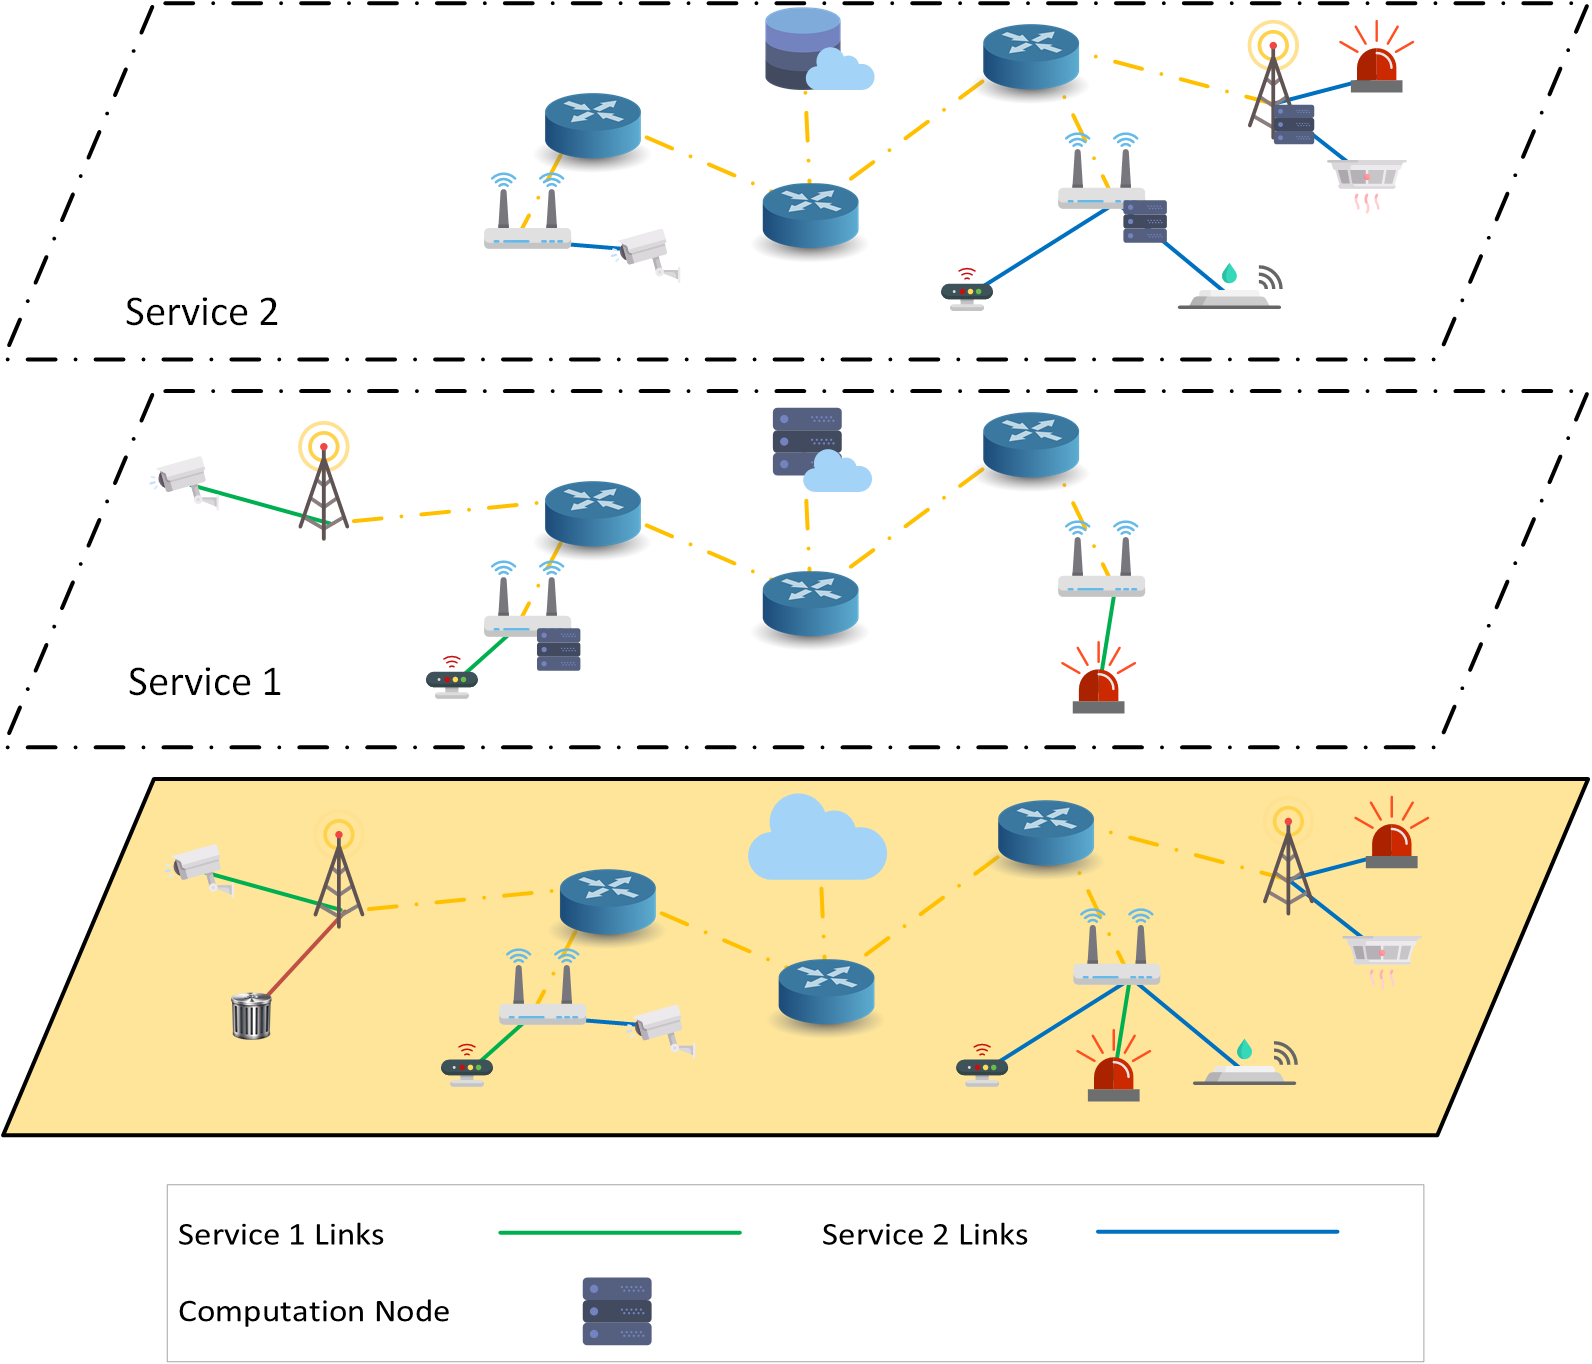
\includegraphics[width=15cm]{graphics/many_to_many/system_model}}
      \caption{دید کلی از مدل سیستم \cref{chap:many_to_many_allocation}}
      \label{fig:many_to_many:system_model}
    \end{figure}
    در این بخش مدل سیستم برای تخصیص منابع پردازشی در شبکه اینترنت اشیاء به صورت چند به چند را توضیح می‌دهیم.
    \cref{fig:many_to_many:system_model} مثالی از مدل سیستم این فصل را نشان می‌دهد که دارای دو سرویس است.
    سرویس اول از یک منبع پردازشی لبه شبکه به همراه منابع پردازشی ابری و سرویس دوم از دو منبع پردازشی لبه شبکه برای پردازش استفاده می‌کند و یکی از مقصد‌های نتایج پردازش‌ها، سرویس‌های ذخیره‌سازی ابری است.

    \cref{tbl:many_to_many:notation} به صورت خلاصه پارامتر‌های استفاده شده در این فصل را معرفی می‌کند.
    باید توجه شود که از تکرار معرفی پارامتر‌هایی که در \cref{chap:one_to_one_allocation} استفاده شده‌اند، صرف نظر شده‌است.
    \begin{table}[h]
      \caption{نماد‌های استفاده شده در \cref{chap:many_to_many_allocation}}
      \begin{tabularx}{\textwidth}{|c|C|} \hline
        نشانه             & توضیح                                                                  \\ \hline
        $I_s$             & مجموعه منابع پردازشی که سرویس $s$ از آن‌ها استفاده می‌کند                \\ \hline
        $I_i$             & مجموعه سرویس‌هایی که منبع پردازشی $i$ به آن‌ها اختصاص پیدا کرده‌است       \\ \hline
        $C_s$             & مجموعه منابع پردازشی که سرویس $s$ می‌تواند از آن‌ها استفاده کند        \\ \hline
        $S_i$             & مجموعه سرویس‌هایی که منبع پردازشی $i$ می‌تواند به آن‌ها اختصاص پیدا کند   \\ \hline
        $Q_s$             & حداکثر تعداد منابع پردازشی که سرویس $s$ مجاز به استفاده از آن‌ها است    \\ \hline
        $Q_i$             & حداکثر تعداد سرویس‌هایی که منبع پردازشی $i$ می‌تواند به آن‌ها اختصاص پیدا کند  \\ \hline
        $d_{i,s}$         & تأخیر منبع پردازشی $i$ برای سرویس $s$                                       \\ \hline
        $d_s^\text{max}$  & بیش‌ترین تاخیر سرویس $s$ بین منابع پردازشی که از آن‌ها استفاده می‌کند         \\ \hline
        $r_{i,s}$         & نرخی که سرویس $s$ برای پردازش به منبع پردازشی $i$ می‌فرستد                   \\ \hline
        $u_{i,s}$         & بخشی از ظرفیت پردازشی منبع پردازشی $i$ که توسط سرویس $s$ استفاده می‌شود      \\ \hline
      \end{tabularx}
      \label{tbl:many_to_many:notation}
    \end{table}
    مانند فصل قبل تابع هدف بهینه سازی از دو قسمت تشکیل می‌شود که قسمت اول تابع نرخ انتخابی سرویس‌ها و قسمت دوم مربوط به تاخیر‌ها است
    \begin{equation}
      U_s = \alpha_s \left ( \omega_s f_r(r_s, R_s) + (1-\omega_s) f_d(d_s^\text{max}) \right ) .
    \end{equation}
    در این رابطه $r_s$ مجموع نرخی است که توسط منابع پردازشی برای سرویس $s$ پردازش می‌شود.
    اگر $r_{i,s}$ را نرخی که توسط منبع پردازشی $i$ برای سرویس $s$ پردازش می‌شود در نظر بگیریم، رابطه زیر برای $r_s$ برقرار است
    \begin{equation}
      r_s = \sum_{i \in C_s}^M r_{i,s} .
    \end{equation}

    چون در این فصل فرض بر این است که هر سرویس می‌تواند از چند منبع پردازشی استفاده کند، بیشترین تاخیر منابع پردازشی مورد استفاده هر سرویس‌ را به عنوان تاخیر آن سرویس در نظر می‌گیریم.
    اگر فرض کنیم $d_{i,s}$ تاخیر پردازش سرویس $s$ در منبع پردازشی $i$ و $d_s^\text{max}$ بیشترین تاخیر سرویس $s$ باشد، $d_s^\text{max}$ باید از همه $d_{i,s}$ها بزرگ‌تر باشد.
    در نتیجه قید زیر باید برای همه منابع پردازشی انتخاب شده توسط سرویس $s$ برقرار باشد
    \begin{equation}\label{eqn:max_delay}
      d_{i,s} < d_s^\text{max}; \forall s \in S, i \in C_s, \delta_{i,s} = 1.
    \end{equation}
    هر کدام از $d_{i,s}$ها مانند فصل قبل از دو بخش تشکیل شده‌اند.
    قسمت اول آن مربوط به تاخیر شبکه است که برابر است با زمانی که طول می‌کشد تا نمونه‌ها به منبع پردازشی برسند به علاوه زمانی که طول می‌کشد نتیجه به مقصد برسد.
    قسمت دوم، تاخیر پردازش نمونه‌ها در منابع پردازشی است.
    این تاخیر برابر زمانی است که طول می‌کشد تا نمونه‌ها پس از رسیدن به منابع پردازشی، پردازششان پایان یابد.
    همانند فصل قبل برای محاسبه تاخیر پردازشی از تئوری صف استفاده می‌کنیم.
    به دلیل این‌که در این فصل فرض بر این است که منابع پردازشی بین چند سرویس ممکن است تقسیم شوند، از مدل $M/M/1$ استفاده می کنیم چرا که در این حالت پردازنده منابع پردازشی بین سرویس‌های آن منبع به اشتراک گذاشته می‌شود.
    در مدل $M/M/1$ میانگین تاخیر $\omega$ از رابطه زیر بدست می‌آید\cite{basic_queueing_sztrik}
    \begin{equation}
      \omega = \frac{1}{\mu-\lambda}.
    \end{equation}

    مانند فصل قبل، ظرفیت پردازشی منبع پردازشی $i$ را با $\varphi_i = \phi_i \nu_i$ نشان می‌دهیم.
    در این فصل متغیر $u_{i,s}$ تعیین می‌کند که چه مقدار از ظرفیت پردازشی منبع پردازشی $i$ به سرویس $s$ اختصاص پیدا می‌کند.
    واضح است که سرویس‌ها نمی‌توانند بیش‌تر از ظرفیت منابع پردازشی از آن‌ها استفاده کنند.
    در نتیجه رابطه زیر برای مقادیر ظرفیت‌های پردازشی تخصیص یافته به سرویس‌ها برای همه منابع پردازشی باید برقرار باشد:
    \begin{equation}
      \sum_{s \in S_i} u_{i,s} \le 1, \forall i \in C.
    \end{equation}
    این رابطه بیان می‌کند که مجموع ظرفیت پردازشی اختصاص داده شده به سرویس ها برای هر منبع پردازشی نباید از ظرفیت کلی آن منبع پردازشی بیشتر باشد.

    مانند \cref{chap:one_to_one_allocation} نرخ سرویس برای سرویس $s$ در منبع پردازشی $i$ از رابطه زیر بدست خواهد آمد
    \begin{equation}
      \mu_{i,s} = \frac{\varphi_i}{F_s} u_{i,s} = \zeta_{i,s} u_{i,s}, \forall s \in S, i \in C_s.
    \end{equation}
    در واقع $\mu_{i,s}$،نرخ اجرا شدن $F_s$ دستورالعمل پردازنده توسط قسمتی از کل ظرفیت پردازنده منبع پردازشی $i$که به وسیله‌ی $u_{i,s}$ مشخص می‌شود است.
    با این تفاسیر رابطه‌ی زیر را برای تاخیر پردازشی سرویس $s$ در منبع پردازشی $i$ وقتی از آن منبع پردازشی استفاده می‌کند می‌توان نوشت
    \begin{equation}
      d_{i,s}^\text{CPU} = \frac{1}{\zeta_{i,s} u_{i,s} - r_{i,s}}.
    \end{equation}
    درنتیجه رابطه زیر برای تاخیر سرویس $s$ در منبع پردازشی $i$ برقرار است
    \begin{equation}
      d_{i,s} = d_{i,s}^\text{net} + \frac{1}{\zeta_{i,s} u_{i,s} - r_{i,s}}.
    \end{equation}
    این رابطه به عنوان قید در یک بهینه سازی محدب قابل استفاده نیست.
    به همین دلیل سعی می‌کنیم تغییراتی در آن ایجاد کنیم تا به یک قید محدب تبدیل شود.
    با توجه به وجود $d_{i,s}^\text{max}$ در تابع هدف بهینه سازی، شرایط بیان شده برای تابع $f_d$ در \cref{chap:one_to_one_allocation} و این‌که \cref{eqn:max_delay} جزء قید‌های مسئله است، می‌توانیم علامت = را با علامت $\le$ جایگزین کنیم
    \begin{equation}
      \frac{1}{\zeta_{i,s} u_{i,s} - r_{i,s}} \le d_{i,s} - d_{i,s}^\text{net}.
    \end{equation}
    چون لگاریتم یک تابع صعودی است، می‌توان بدون مشکلی از دو طرف نامساوی، لگاریتم گرفت و جهت علامت نامساوی تغییری نکند.
    با لگاریتم گرفتن از طرفین می‌توان قید مناسب برای استفاده در بهینه سازی محدب را بدست آورد
    \begin{equation}\label{eqn:delay_inequality}
      - \log (\zeta_{i,s} u_{i,s} - r_{i,s}) - \log (d_{i,s} - d_{i,s}^\text{net}) \le 0.
    \end{equation}
    دلیل محدب بودن \cref{eqn:delay_inequality} این است که $\zeta_{i,s} u_{i,s} - r_{i,s}$ و $d_{i,s} - d_{i,s}^\text{net}$ هر دو تابع محدب هستند.
    همچنین تابع $-\log$ هم یک تابع محدب است.
    با توجه به قضیه ترکیب توابع محدب \cite{boyd2004convex}، \cref{eqn:delay_inequality} یک قید محدب است.

    با توجه به آنچه که تا این جا گفته شد،‌ می‌توان مسئله بهینه سازی را به صورت زیر نوشت
    \begin{subequations}\label{eqn:optimization2}
      \begin{align}
        \underset{r_{i,s}, u_{i,s}, \delta_{i,s}}{\text{maximize}} \qquad & \sum_{s=1}^N \alpha_s \left (\omega_s f_r(r_s, R_s) + (1-\omega_s) f_d(d_s^\text{max}) \right ) \\
        \text{\lr{subject  to}} \qquad & \nonumber \\
        & r_s = \sum_{i \in S_i} r_{i,s}, \forall s \in S \\
        & 0 \le r_{i,s}, \forall s \in S, i \in C_s \label{eqn:rate_positiveness2} \\
        & r_{i,s} \le \eta \zeta_{i,s} u_{i,s}, \forall s \in S, i \in C_s \label{eqn:rate_saturation2} \\
        & u_{i,s} \le \delta_{i,s}, \forall s \in S, i \in C_s \label{eqn:u_le_delta} \\
        & d_{i,s} \le d_s^\text{max}, \forall s \in S, i \in C_s, \delta_{i,s}=1 \\
        &- \log \left((\zeta_{i,s} u_{i,s} - r_{i,s}) (d_{i,s} - d_{i,s}^\text{net}) \right ) \le 0, \forall s \in S, i\in C_s, \delta_{i,s}=1 \\
        & \sum_{s \in S_i} u_{i,s} \le 1, \forall i \in C \label{eqn:sum_of_utiliztion} \\
        & \sum_{s \in S_i} \delta_{i,s} \le Q_i, \forall i \in C \label{eqn:computation_quota} \\
        & \sum_{i \in C_s} \delta_{i,s} \le Q_s, \forall s \in S \label{eqn:service_quota} \\
        & \delta_{i,s} \in \{0, 1\}, \forall s \in S, i \in C_s
      \end{align}
    \end{subequations}
    در این مسئله
    قید \eqref{eqn:u_le_delta} باعث می‌شود که زمانی که سرویس $s$ از منبع پردازشی $i$ استفاده نمی‌کند $u_{i,s}=0$ باشد و در صورت استفاده $u_{i,s}<1$ باشد.
    باید توجه کرد که قیدهای \cref{eqn:rate_positiveness2} و \cref{eqn:rate_saturation2} باعث می‌شوند که $u_{i,s}$ها مثبت باشند.
    قید \eqref{eqn:sum_of_utiliztion} برای این در بهینه سازی حضور دارد که میزان استفاده از منابع پردازشی نمی‌تواند بیشتر از ظرفیت آن‌ها باشد.
    قید \eqref{eqn:computation_quota} نشان دهنده‌ی حداکثر تعداد سرویس‌هایی است که یک منبع پردازشی می‌تواند به آن‌ها اختصاص پیدا کند.
    قید \eqref{eqn:service_quota} برای محدود کردن حداکثر تعداد منابع پردازشی که یک سرویس می‌تواند استفاده کند است.
    
    مانند فصل قبل، این مسئله بهینه سازی هم یک مسئله برنامه‌ریزی غیرخطی عدد صحیح مخلوط می‌باشد که پیدا کردن جواب بهینه آن ساده نیست.
    به همین دلیل در بخش بعدی یک الگوریتم برای پیدا کردن جواب زیر بهینه آن معرفی می‌کنیم.

  \section{معرفی الگوریتم زیر بهینه}
    از آن‌جایی که پیدا کردن مقدار بهینه مسئله \eqref{eqn:optimization2} نیاز به زمان طولانی دارد، برای پیدا کردن جواب آن یک الگوریتم مبتنی بر تکرار معرفی می‌کنیم که در زمان کوتاهی به جواب می‌رسد.
    در هر تکرار الگوریتم، برای هر سرویس، یک تغییر در منابع پردازشی اختصاص یافته به آن سرویس ایجاد می‌کنیم.
    این تغییر می‌تواند حذف کردن، اضافه کردن یا جابه‌جایی منابع پردازشی آن سرویس باشد به شرطی که پس از تغییر، قید‌های حداکثر تعداد سرویس‌های منابع پردازشی و حداکثر تعداد منابع پردازشی سرویس برقرار باشند.
    این کار را در هر تکرار برای همه‌ی سرویس‌ها انجام می‌دهیم و تغییر ایجاد شده در تابع هدف بهینه‌سازی با مرحله قبل را درنظر می‌گیریم.
    پس از انجام این کار، تغییری که بیشترین افزایش را در تابع هدف بهینه‌سازی دارد به تخصیص منابع اعمال می‌کنیم.
    این الگوریتم تا زمانی که مقدار افزایش تابع هدف بهینه سازی در هر مرحله بیشتر از مقدار مشخص $\epsilon$ باشد ادامه می‌دهیم.

    \cref{alg:suboptimal_algorithm} به صورت خلاصه مراحل این الگوریتم را نشان می‌دهد.
    \cref{alg:loop} باعث می‌شود که الگوریتم تاز مانی که تغییرات مرحله قبل بیش از $\epsilon$ باشد، ادامه پیدا کند.
    سپس در \cref{alg:set_d} مقدار تغییرات در مرحله جدید برابر صفر قرار داده می‌شود.
    در \cref{alg:service_loop} همه سرویس‌ها مورد بررسی قرار می‌گیرند.
    برای بررسی هر سرویس در \cref{alg:computation_resources}،همه منابع پردازشی ممکن $c_1$ و $c_2$ بررسی می‌شوند.
    $c_1$ منبع پردازشی است که از مراحل قبل به سرویس مورد بررسی اختصاص پیدا کرده و حذف شدن آن را بررسی می‌کنیم و $c_2$ منبع پردازشی است که اختصاص پیدا کردن آن به سرویس را بررسی می‌کنیم که هرکدام می‌تواند تهی باشد.
    در واقع در هر بار بررسی، منبع پردازشی $c_1$ را از مجموعه منابع پردازشی اختصاص پیدا کرده به سرویس حذف کرده و $c_2$ را به آن اضافه می‌کنیم.
    اگر منبع پردازشی $c_2$ تهی باشد یعنی فقط منبع پردازشی $c_1$ از منابع اختصاص پیدا کرده به سرویس حذف می‌شود و اگر $c_1$ تهی باشد یعنی فقط منبع پردازشی $c_2$ به سرویس اختصاص پیدا می‌کند.
    برای این کار در \crefrange{alg:temp_add1}{alg:temp_add3} این تغییر را به صورت موقت در اختصاص منابع اعمال می‌کنیم و در \crefrange{alg:temp_remove1}{alg:temp_remove3} اختصاص منابع را به حالت قبل باز می‌گردانیم.
    پس از بررسی معتبر بودن این تغییرات در \cref{alg:quota_validity}، در \cref{alg:solve_new_assignment} مقدار بهینه تابع هدف با منابع اختصاص یافته جدید محاسبه می‌شود و نتیجه در $\nu'$ قرار می‌گیرد.
    در \cref{alg:optimization_value_comparison}، $\nu'$ با بیشترین مقداری که تا الان بدست آمده، $\nu$، مقایسه می‌شود و در صورتی که $\nu'$ از آن بیشتر بود، مقادیر $\nu$، $d$ و بهترین تخصیص منابع به روز رسانی می شوند (\crefrange{alg:best_update1}{alg:best_update5}).
    در پایان هر مرحله تخصیص منابعی که بیشتری افزایش را در تابع هدف مسئله داشته، اعمال می‌شود (\crefrange{alg:update_assignment1}{alg:update_assignment3}).

    \begin{latin}
      \begin{algorithm}[]
        \caption{Auction ‌Based Resource Assignment Algorithm}
        \label{alg:suboptimal_algorithm}
        \begin{algorithmic}[1]
          \State{$\nu \gets -\infty$}
          \State{$d \gets \infty$}
          \While{$d > \epsilon$} \label{alg:loop}
            \State{$d \gets 0$} \label{alg:set_d}
            \For {$s \in S$} \label{alg:service_loop}
              \For {$(c_1,c_2) \in (I_s \cup \{\_\}) \times ((C_s \setminus I_s) \cup \{\_\}) $} \label{alg:computation_resources}
                \If{$s \in S_{c_2}$}
                  \State{$I_s \gets (I_s \setminus \{c_1\}) \cup \{c_2\}$} \label{alg:temp_add1}
                  \State{$I_{c_1} \gets I_{c_1} \setminus \{s\}$} \label{alg:temp_add2}
                  \State{$I_{c_2} \gets I_{c_2} \cup \{s\}$} \label{alg:temp_add3}
                  \If{$|I_s| \le Q_s|$ and $|I_{c_2}| \le Q_{c_2}|$} \label{alg:quota_validity}
                    \State{$\nu' = $ Obtimization Objective Value} \label{alg:solve_new_assignment}
                    \If {$\nu' > \nu$} \label{alg:optimization_value_comparison}
                      \State{$d \gets d + \nu' - \nu$} \label{alg:best_update1}
                      \State{$\nu \gets \nu'$} \label{alg:best_update2}
                      \State{$s^\text{new} \gets s$} \label{alg:best_update3}
                      \State{$c_1^\text{new} \gets c_1$} \label{alg:best_update4}
                      \State{$c_2^\text{new} \gets c_2$} \label{alg:best_update5}
                    \EndIf
                  \EndIf
                  \State{$I_s \gets (I_s \setminus \{c_2\}) \cup \{c_1\}$} \label{alg:temp_remove1}
                  \State{$I_{c_2} \gets I_{c_2} \setminus \{s\}$} \label{alg:temp_remove2}
                  \State{$I_{c_1} \gets I_{c_1} \cup \{s\}$} \label{alg:temp_remove3}
                \EndIf
              \EndFor
            \EndFor
            \State{$I_s^\text{new} \gets (I_s^\text{new} \setminus \{c_1^\text{new}\}) \cup \{c_2^\text{new}\}$} \label{alg:update_assignment1}
            \State{$I_{c_1}^\text{new} \gets I_{c_1}^\text{new} \setminus \{s^\text{new}\}$} \label{alg:update_assignment2}
            \State{$I_{c_2}^\text{new} \gets I_{c_2}^\text{new} \cup \{s^\text{new}\}$} \label{alg:update_assignment3}
          \EndWhile
        \end{algorithmic}
      \end{algorithm}
    \end{latin}

    \subsection{بررسی پیچیدگی الگوریتم}
      در ابتدای‌شروع الگوریتم، نرخ انتخابی همه‌ی سرویس‌ها صفر است و هیچ منبع پردازشی اختصاص پیدا نکرده‌است.
      در نتیجه مقدار تابع هدف بهینه سازی $-\sum_{s=1}^N \alpha_s \omega_s R_s$ می‌باشد.
      علاوه براین تابع هدف بهینه‌سازی همواره یک عدد منفی است.
      با در نظر گرفتن این‌که در هر تکرار، مقدار تابع هدف حداقل به اندازه‌ی $\epsilon$ افزایش پیدا می‌کند، تعداد تکرار‌های الگوریتم نمی‌تواند بیش از $\sum_{s=1}^N  \alpha_s \omega_s R_s / \epsilon$  باشد.
      
      اگر فرض کنیم در مرحله‌ای دلخواه از این الگوریتم سرویس $s$ به $m$ منبع پردازشی اختصاص پیدا کرده باشد و $m'$ تعداد منابع پردازشی اختصاص پیدا نکرده به سرویس $s$ باشد، باید $(m+1) \times (m'+1) - 1$ بار مسئله بهینه‌سازی برای سرویس $s$ حل شود.
      در نتیجه می‌توان نتیجه گرفت که تعداد دفعاتی که مسئله بهینه سازی در هر بار تکرار الگوریتم حل می‌شود، کم‌تر از $N(M+1)^2$ است.
      در نتیجه تعداد دفعاتی که مسئله بهینه سازی در کل الگوریتم حل می‌شود کم‌تر از $N(M+1)^2 \sum_{s=1}^N  \alpha_s \omega_s R_s / \epsilon$ است.
      از این رابطه واضح است که با افزایش $\epsilon$ انتظار می‌رود الگوریتم زود‌تر پایان یابد.
      باید توجه داشت که $(m+1) \times (m'+1) - 1$ حد بالای تعداد دفعات حل شدن مسئله بهینه‌سازی برای هر سرویس را نشان می‌دهد و محدود بودن انتخاب‌های سرویس‌ها و منابع پردازشی(مجموعه‌های $S$ و $C$ برای هر سرویس و منبع پردازشی) باعث می‌شود که تعداد واقعی، کم‌تر از این تعداد باشد.

  \section{نتایج شبیه‌سازی}
    برای شبیه سازی این قسمت از محیطی مانند فصل قبل کمک گرفتیم.
    در همه موارد، شبیه سازی‌ها ۲۰ بار تکرار شده‌اند و نتایج میانگین آورده شده‌است.
    فرض شده‌است که سرویس‌ها و منابع پردازشی به صورت تصادفی در یک دایره با شعاع ۱۰۰ متر پراکنده شده‌اند و توپولوژی شبکه و سایر پارامتر‌ها مانند فصل قبل در نظر گرفته شده‌اند.
    
    فرض می‌کنیم تعداد سرویس‌ها $N=15$ باشد و تعداد منابع پردازشی لبه شبکه ($M$) از ۱۲ تا ۲۰ تغییر کند.
    مطابق فصل قبل، دو سناریو با و بدون حضور منبع پردازشی ابری را در نظر می‌گیریم و میانگین هزینه سرویس‌ها($-U/N$) را رسم می‌کنیم.
    انتظار داریم که با افزایش تعداد منابع پردازشی، میانگین هزینه سرویس‌ها کاهش پیدا کند. چرا که قدرت پردازشی بیشتری در شبکه وجود دارد و می‌تواند باعث کاهش تاخیر یا اختلاف نرخ مطلوب و نرخ بهینه شود.

    نتیجه این شبیه‌سازی در \cref{fig:many_to_many:sim6} آوده شده‌است.
    برای مقایسه نتایج با روش فصل قبل (تخصیص منابع مبتنی بر مزایده) مقایسه شده‌اند.
    با توجه به این که در روش تخصیص منابع مبتنی بر مزایده، تعداد منابع پردازشی باید بیش‌تر از تعداد سرویس‌ها باشد، در دو حالت نتایج این روش محاسبه شده‌است.
    در حالت اول تعداد سرویس‌ها در هر دو روش برابر است به همین دلیل تعداد منابع پردازشی باید بیش‌تر از ۱۵ باشد.
    در حالت دوم تعداد سرویس‌ها از حداقل تعداد منابع پردازشی کم‌تر است به همین دلیل در محدوده منابع پردازشی روش این فصل مقایسه آورده شده‌است.
    همانطور که در شکل هم مشخص است الگوریتم ارائه شده در این فصل نتایج بسیار بهتری ارائه می‌دهد.
    هم‌چنین با افزایش تعداد منابع پردازشی، میانگین هزینه سرویس‌ها کاهشی است.
    علاوه بر این، میانگین هزینه‌ی سرویس‌های سناریوای که منبع پردازشی ابری در آن وجود داشت، همواره کم‌تر از سناریوی بدون منبع پردازش ابری است.
    دلیلش آن است که هرچه تعداد منابع پردازشی بیشتر باشد، ظرفیت پردازشی کل بیشتر می‌شود و برای سرویس‌ها انتخاب بیش‌تری وجود دارد.
    همچنین، با افزایش تعداد منابع پردازشی لبه شبکه، اختلاف این دو سناریو کاهش پیدا می‌کند تا در تعداد ۲۰ منبع پردازشی لبه شبکه، تقریبا صفر می‌شود.
    دلیلش آن است که با افزایش منابع پردازشی لبه شبکه همه پردازش‌ها در لبه شبکه انجام شده و تاثیر وجود منبع پردازشی ابری در میانگین هزینه‌ها به صفر می‌رسد.

    \begin{figure}[]
      \centerline{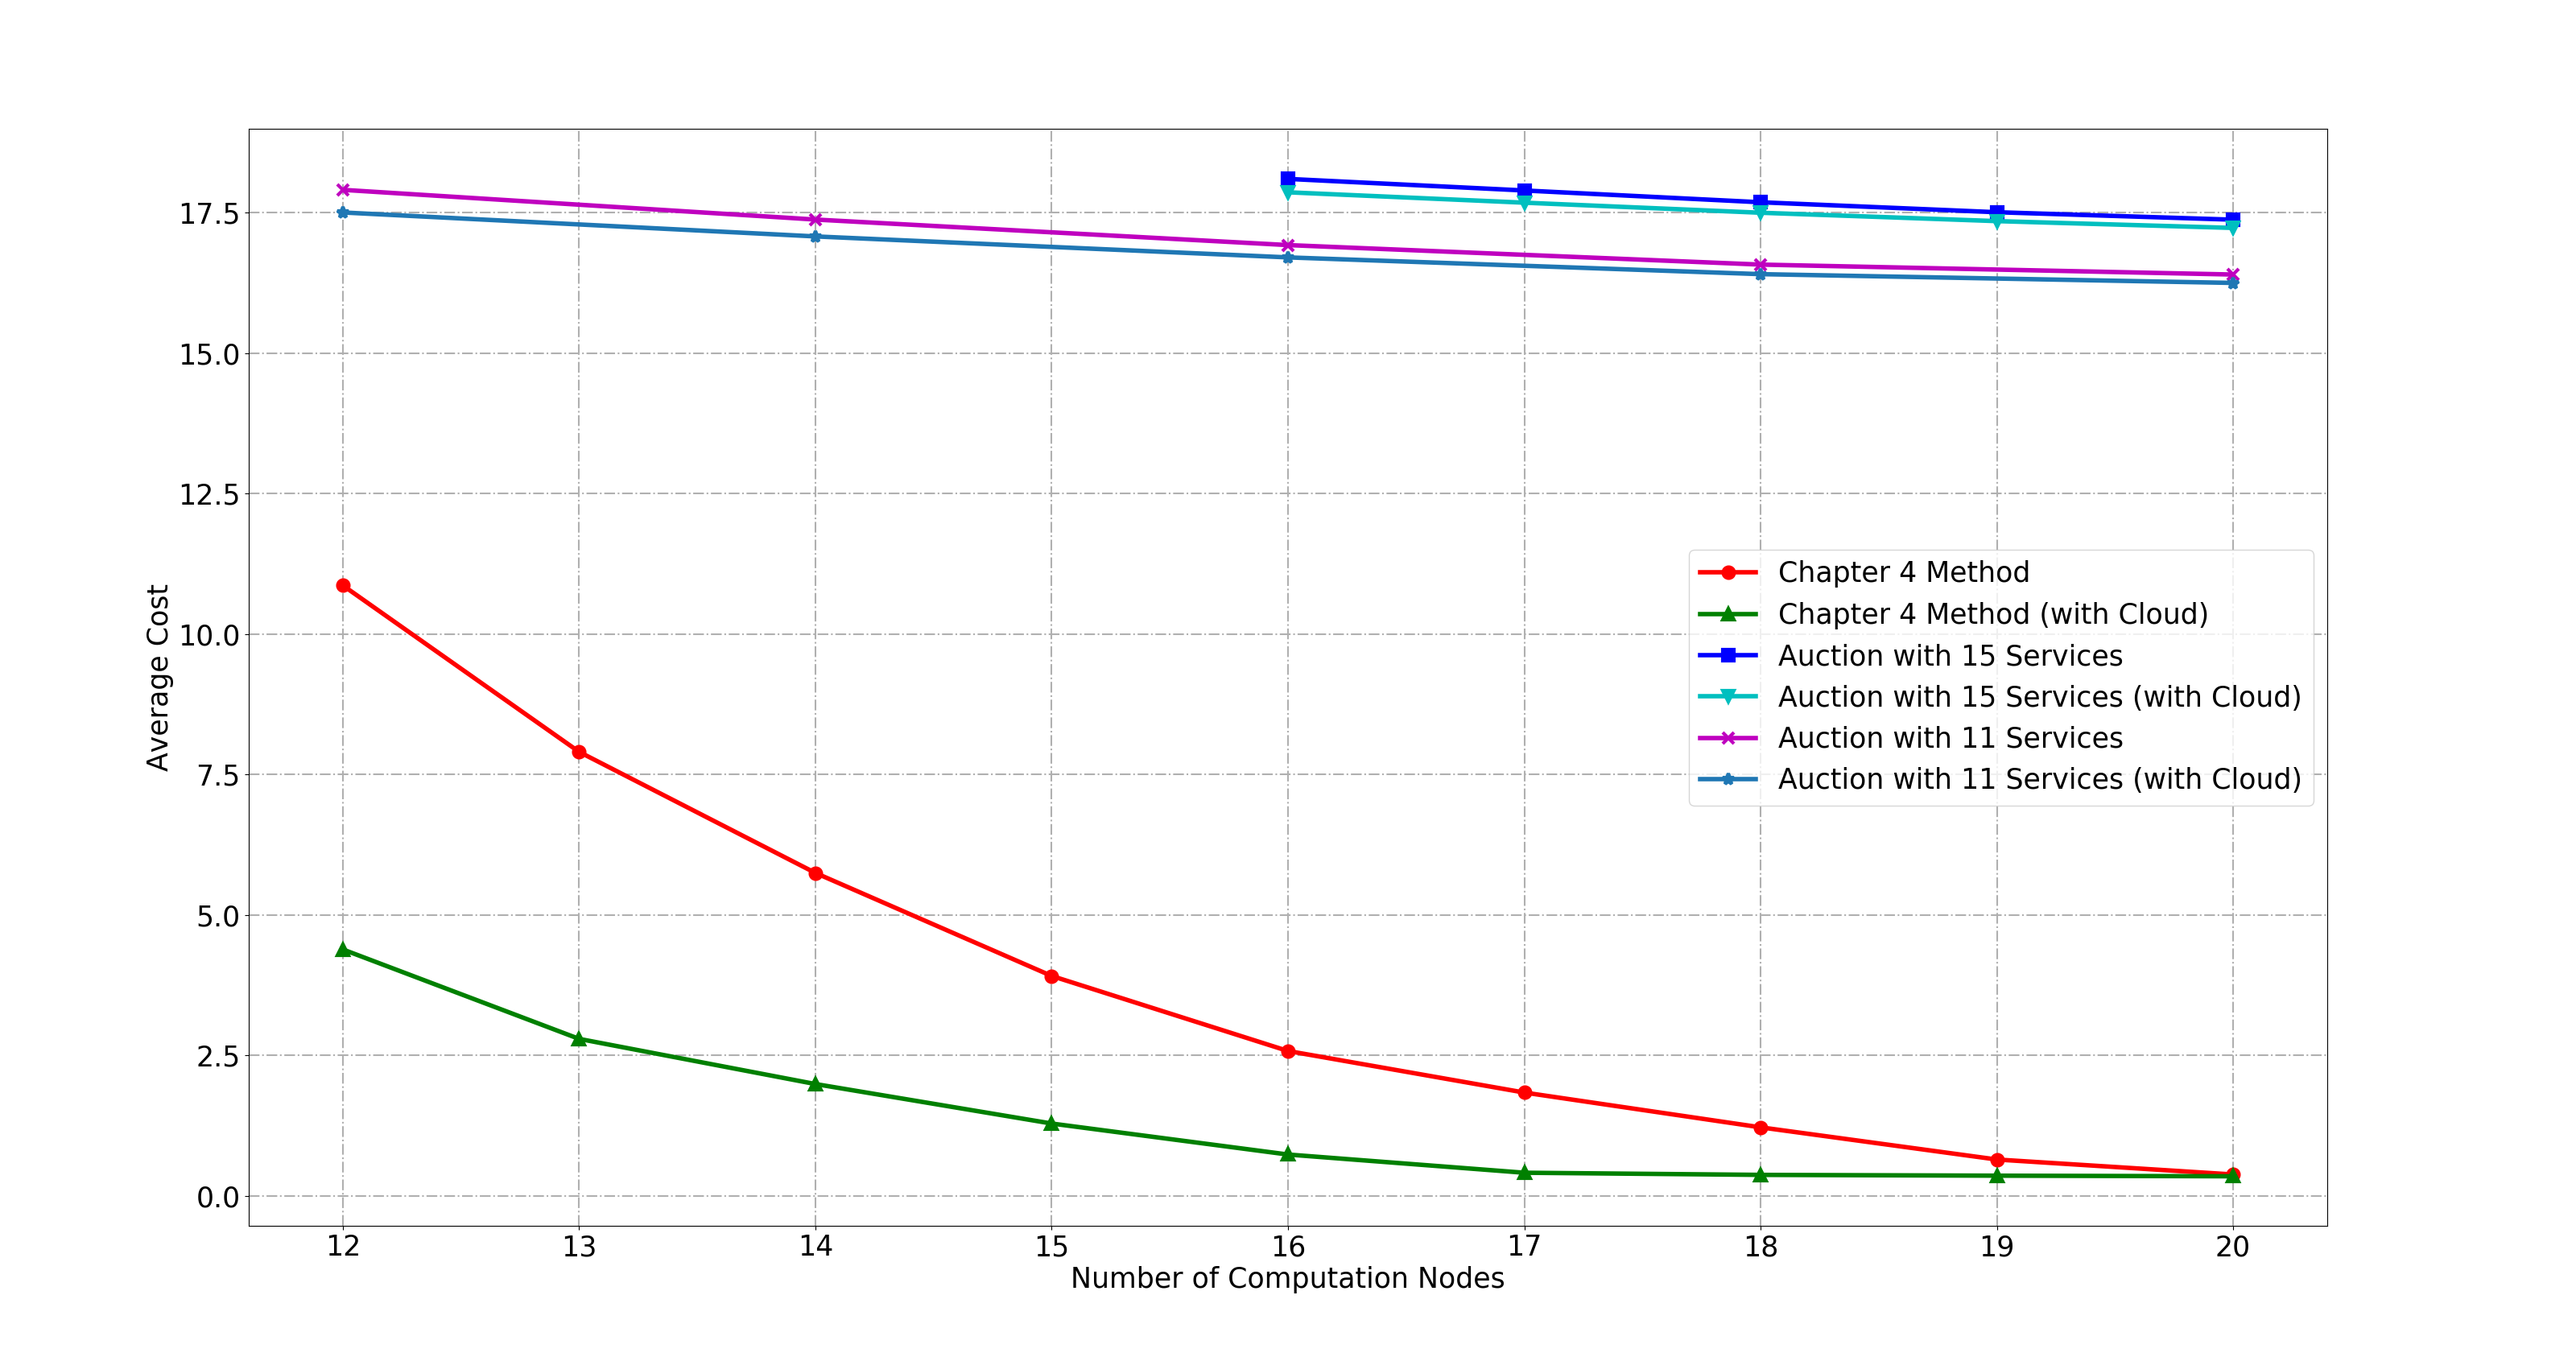
\includegraphics[width=17cm]{graphics/many_to_many/sim_6}}
      \caption{میانگین هزینه سرویس‌ها در برابر تعداد منابع پردازشی در لبه شبکه}
      \label{fig:many_to_many:sim6}
    \end{figure}

    اثر پارامتر $\beta$ در این روش تخصیص منابع در \cref{fig:many_to_many:sim7} بررسی شده‌است.
    در این شکل اثر $\beta$ روی اختلاف نرخ بهینه و مطلوب و بیشترین تاخیر برای یک سرویس در بازه $\beta\in[30, 70]$ رسم شده‌است.
    همان‌طور که بیان شد $\beta$ نسبت اهمیت تاخیر به اختلاف نرخ بهینه و مطلوب است.
    در نتیجه انتظار داریم با افزایش $\beta$ اختلاف نرخ، افزایش پیدا کرده و تاخیر کاهش پیدا کند که شکل هم همین را نشان می‌دهد.
    
    \begin{figure}[]
      \centerline{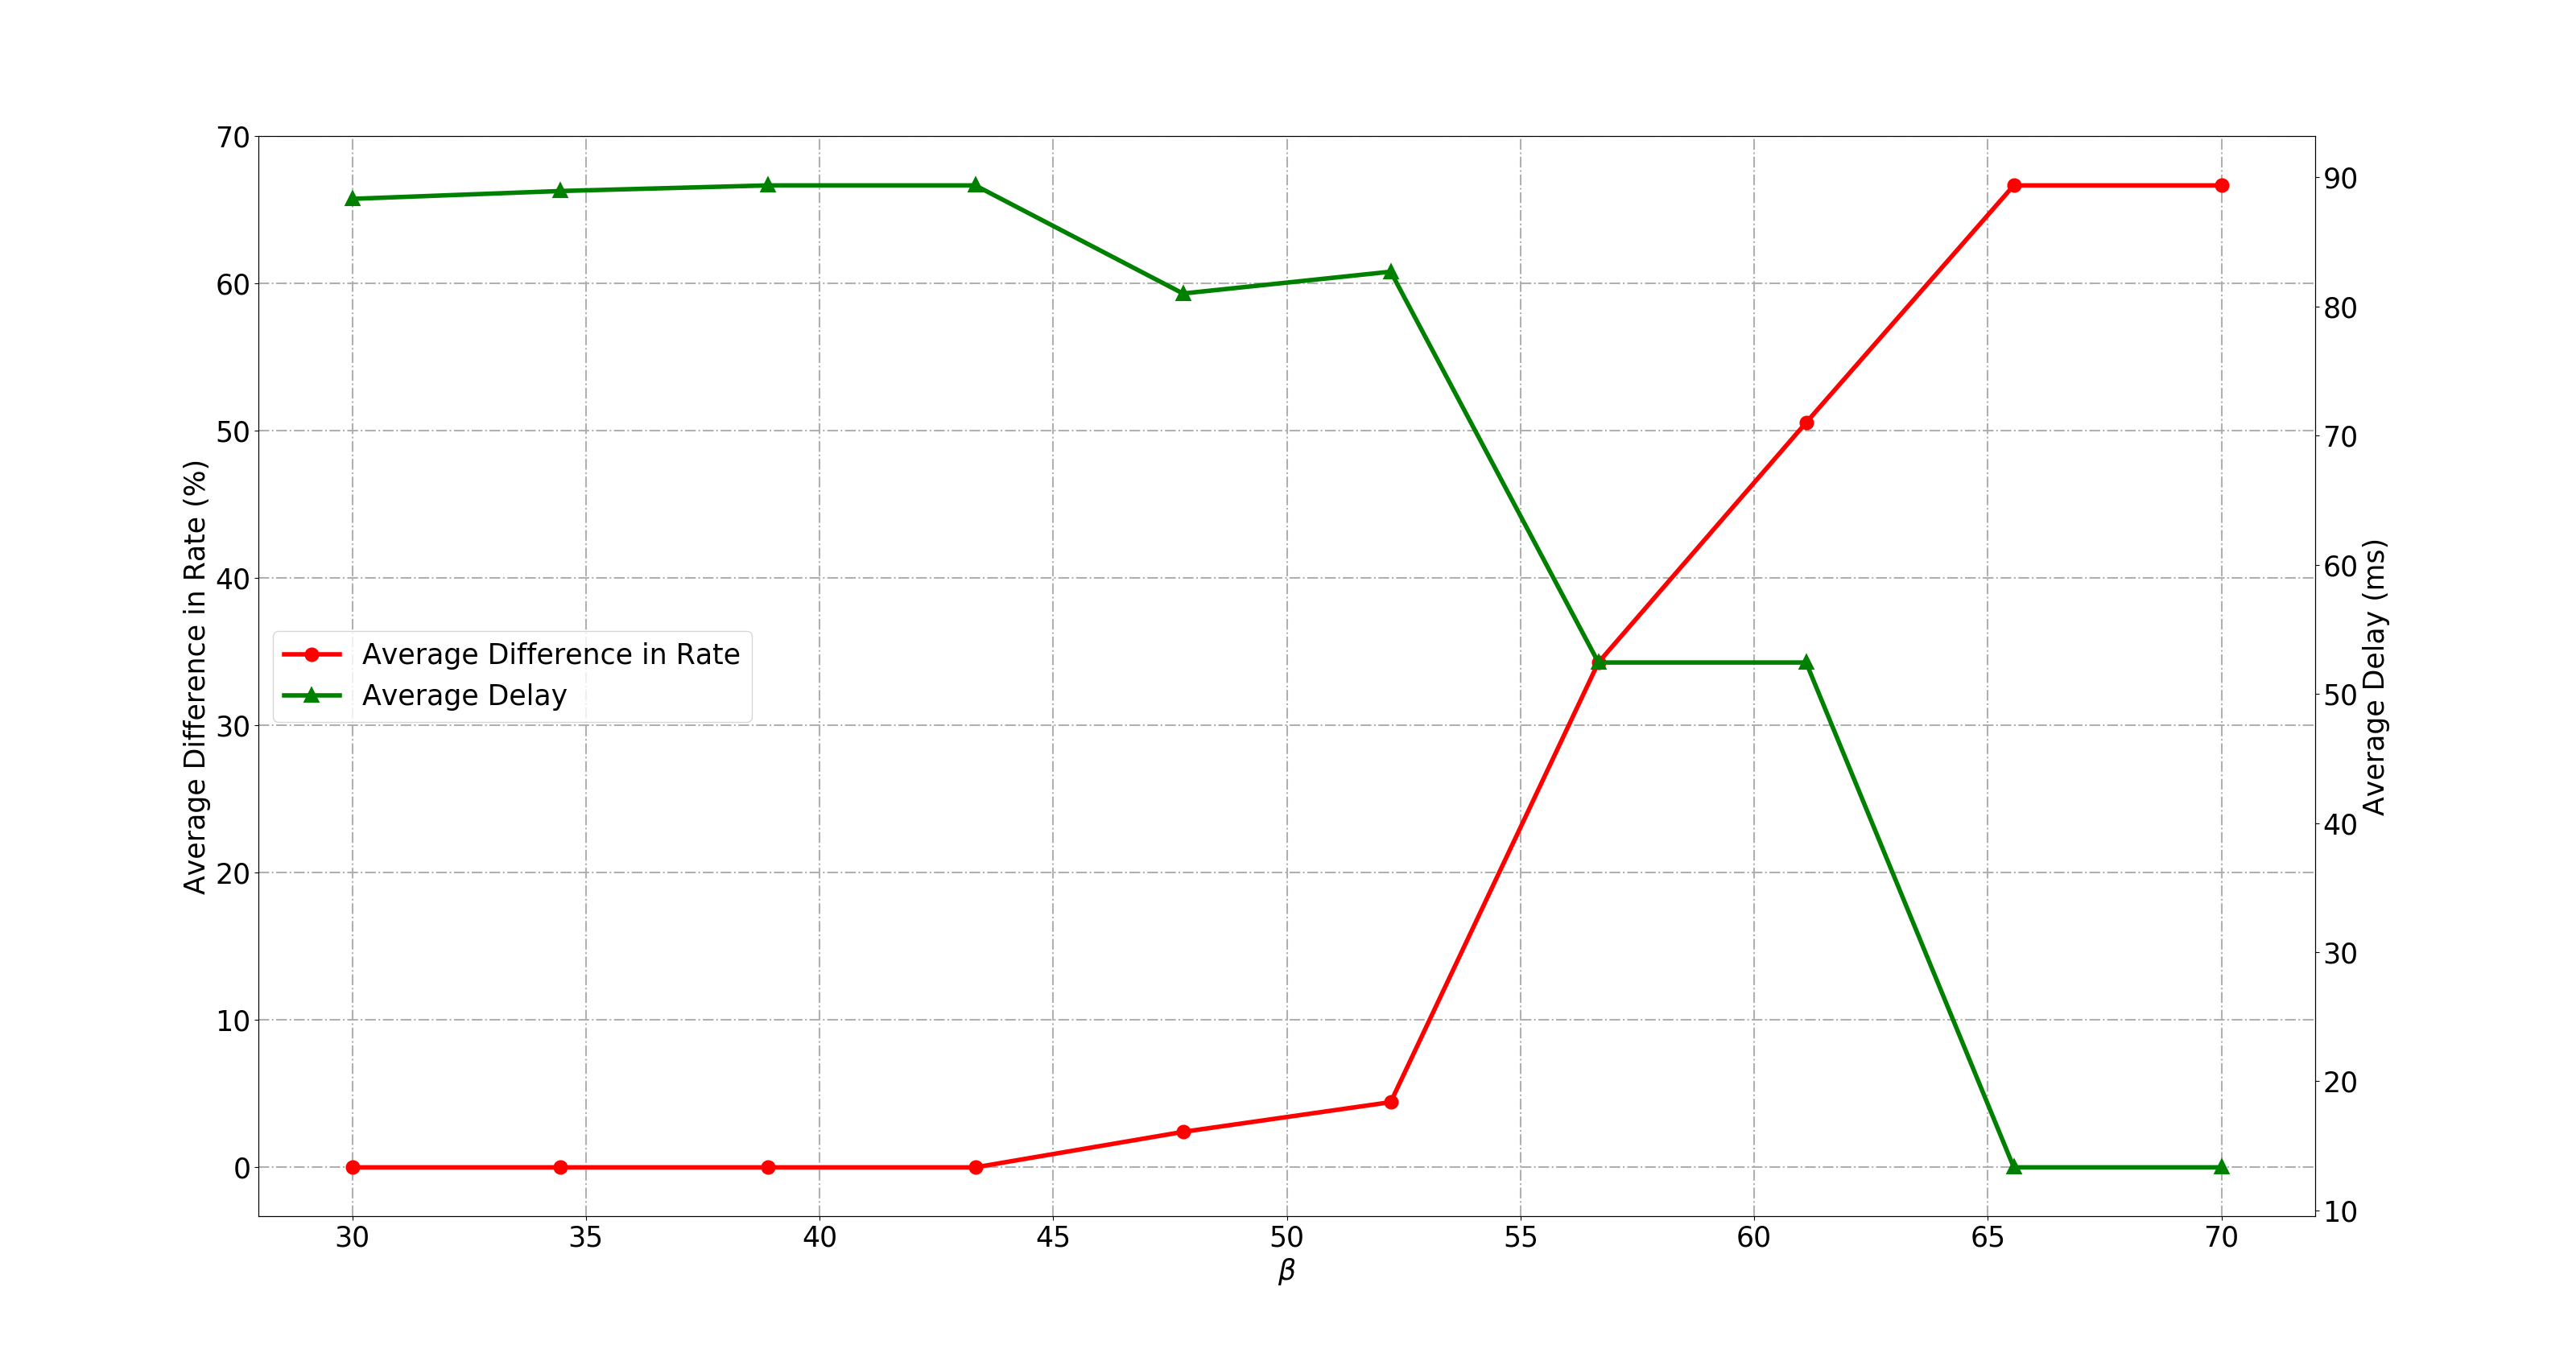
\includegraphics[width=17cm]{graphics/many_to_many/sim_7}}
      \caption{تاثیر $\beta$ بر تاخیر و اختلاف نرخ بهینه با نرخ مطلوب برای یک سرویس}
      \label{fig:many_to_many:sim7}
    \end{figure}

    در \cref{fig:many_to_many:sim8} تاثیر $\alpha_s$ بر روی هزینه یک سرویس بررسی شده‌است.
    به دلیل تاثیر مستقیم $\alpha_s$ در $U_s$، مقدار $-U_s/\alpha_s$ رسم شده‌است.
    افزایش $\alpha_s$ باعث افزایش تاثیر $U_s$ در تابع هدف بهینه سازی می‌شود.
    پس انتظار داریم، افزایش $\alpha_s$ باعث کاهش $-U_s/\alpha_s$ بشود.
    این کاهش معادل کاهش تاخیر و اختلاف نرخ بهینه و مطلوب سرویس $s$ است.

    \begin{figure}[]
      \centerline{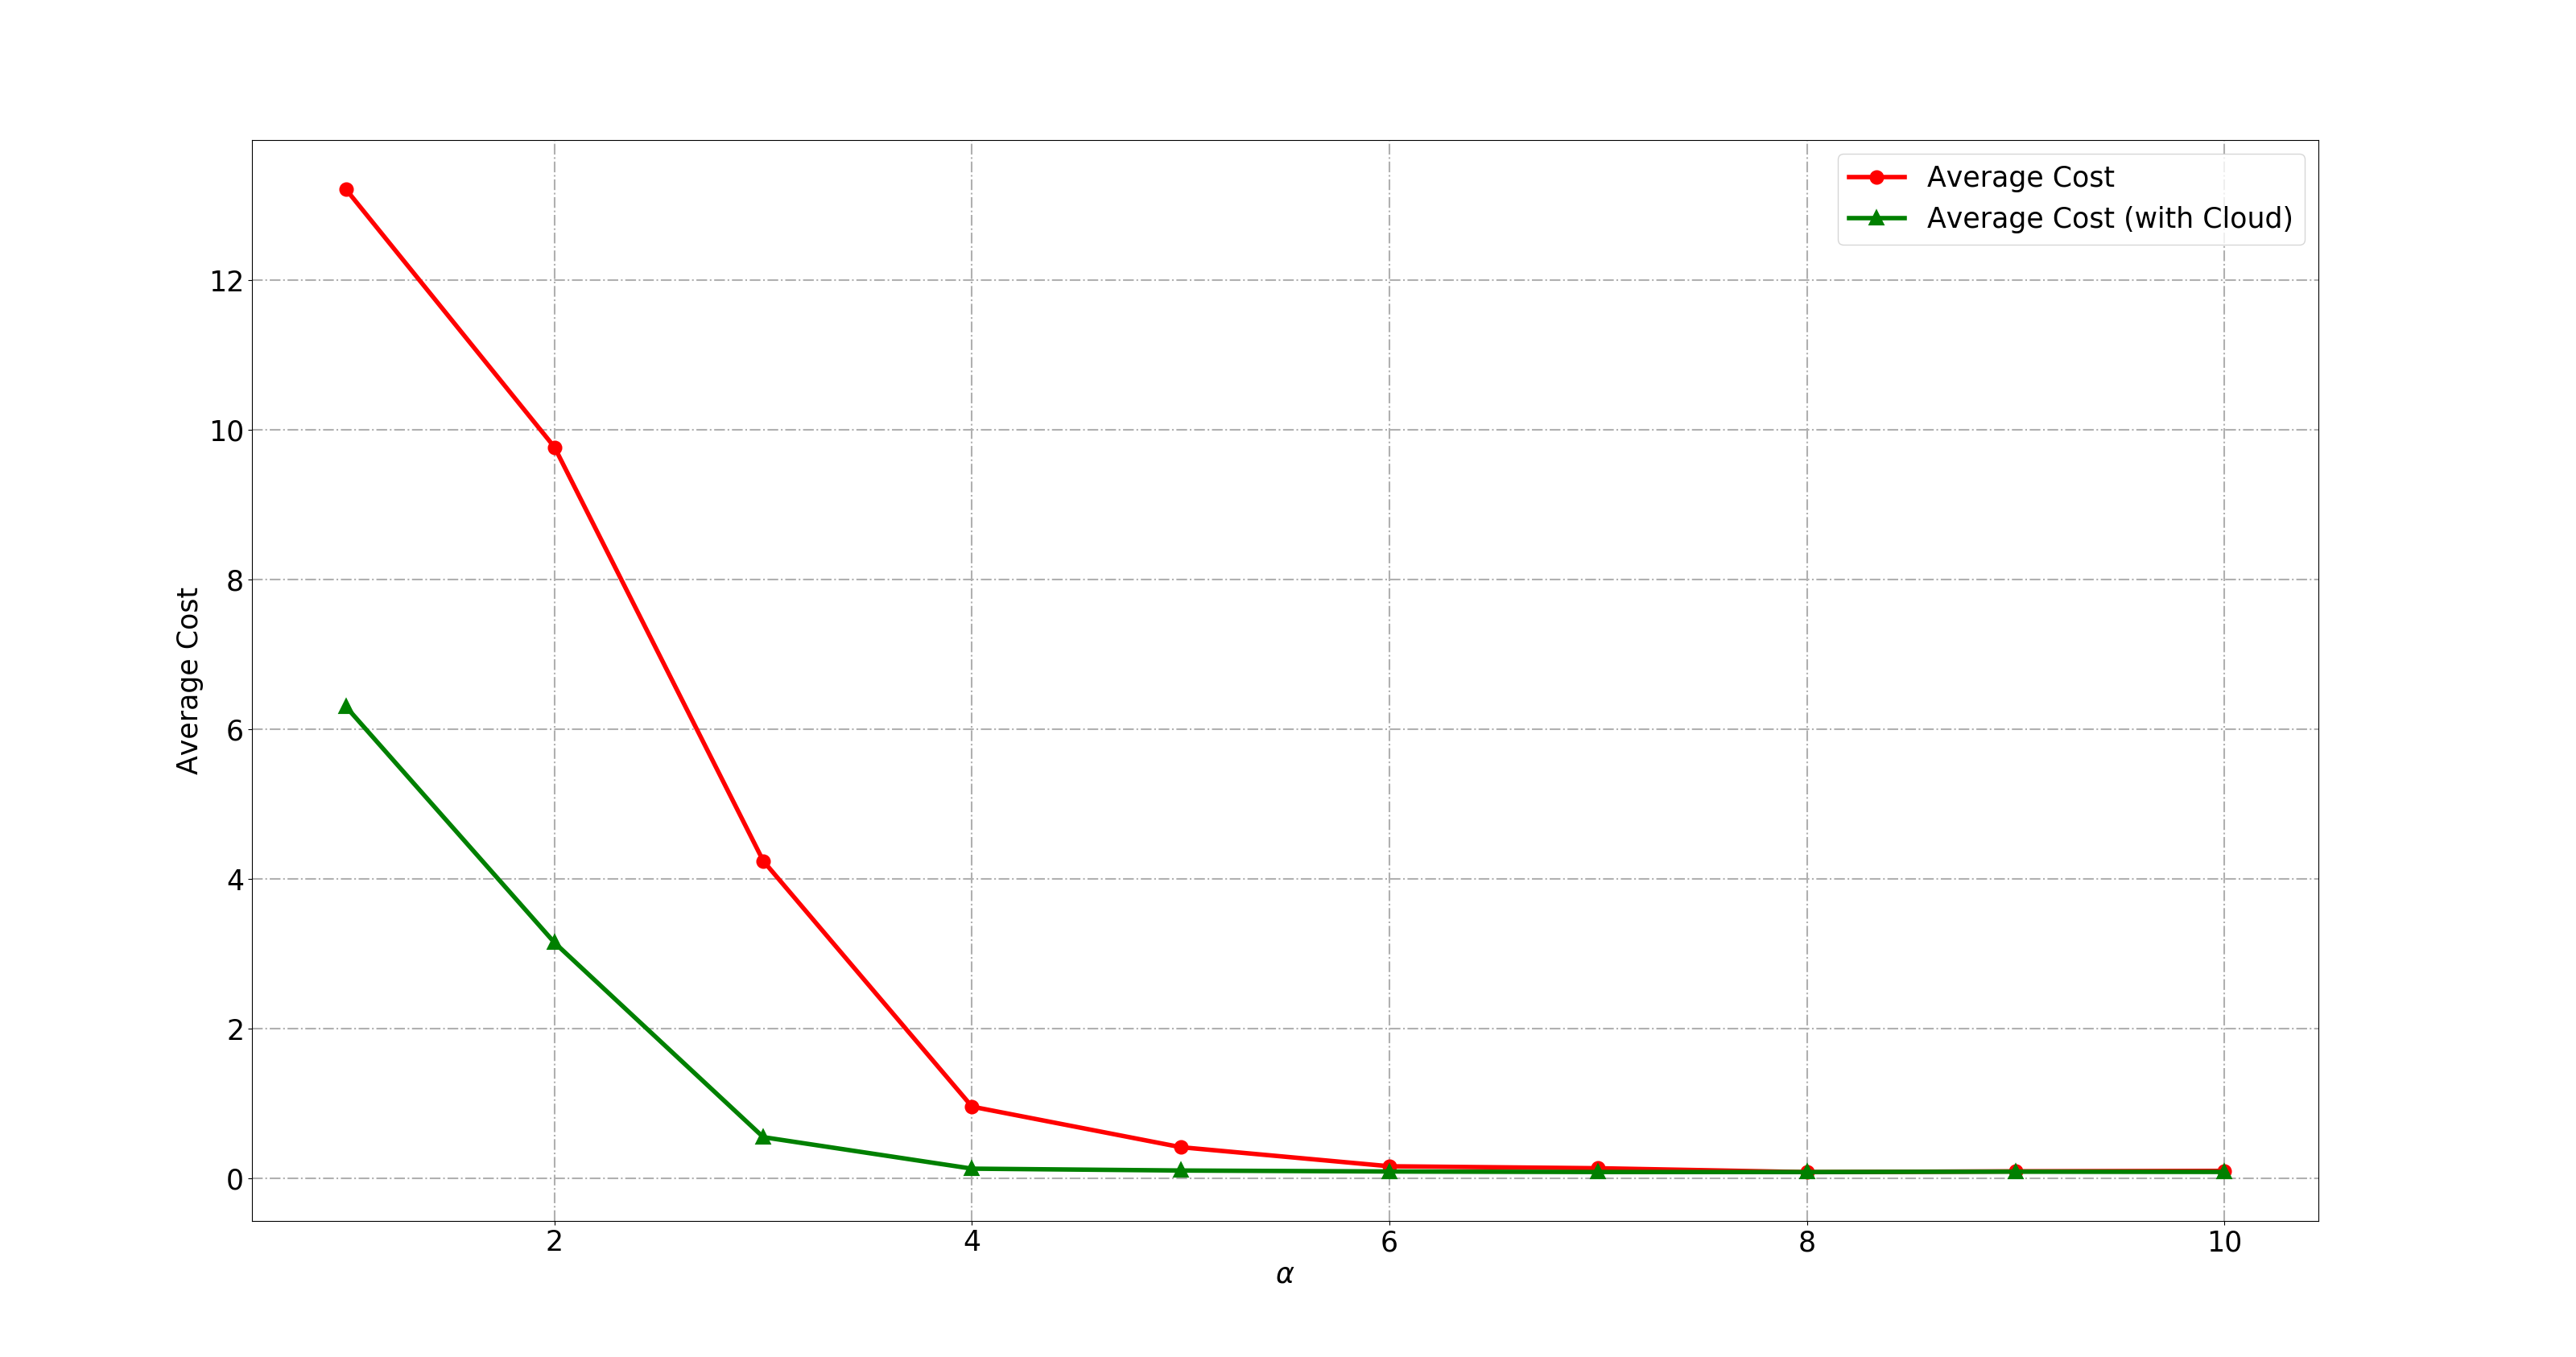
\includegraphics[width=17cm]{graphics/many_to_many/sim_8}}
      \caption{تاثیر $\alpha$ بر میانگین هزینه سرویس‌ها}
      \label{fig:many_to_many:sim8}
    \end{figure}

    \begin{figure}[]
      \centerline{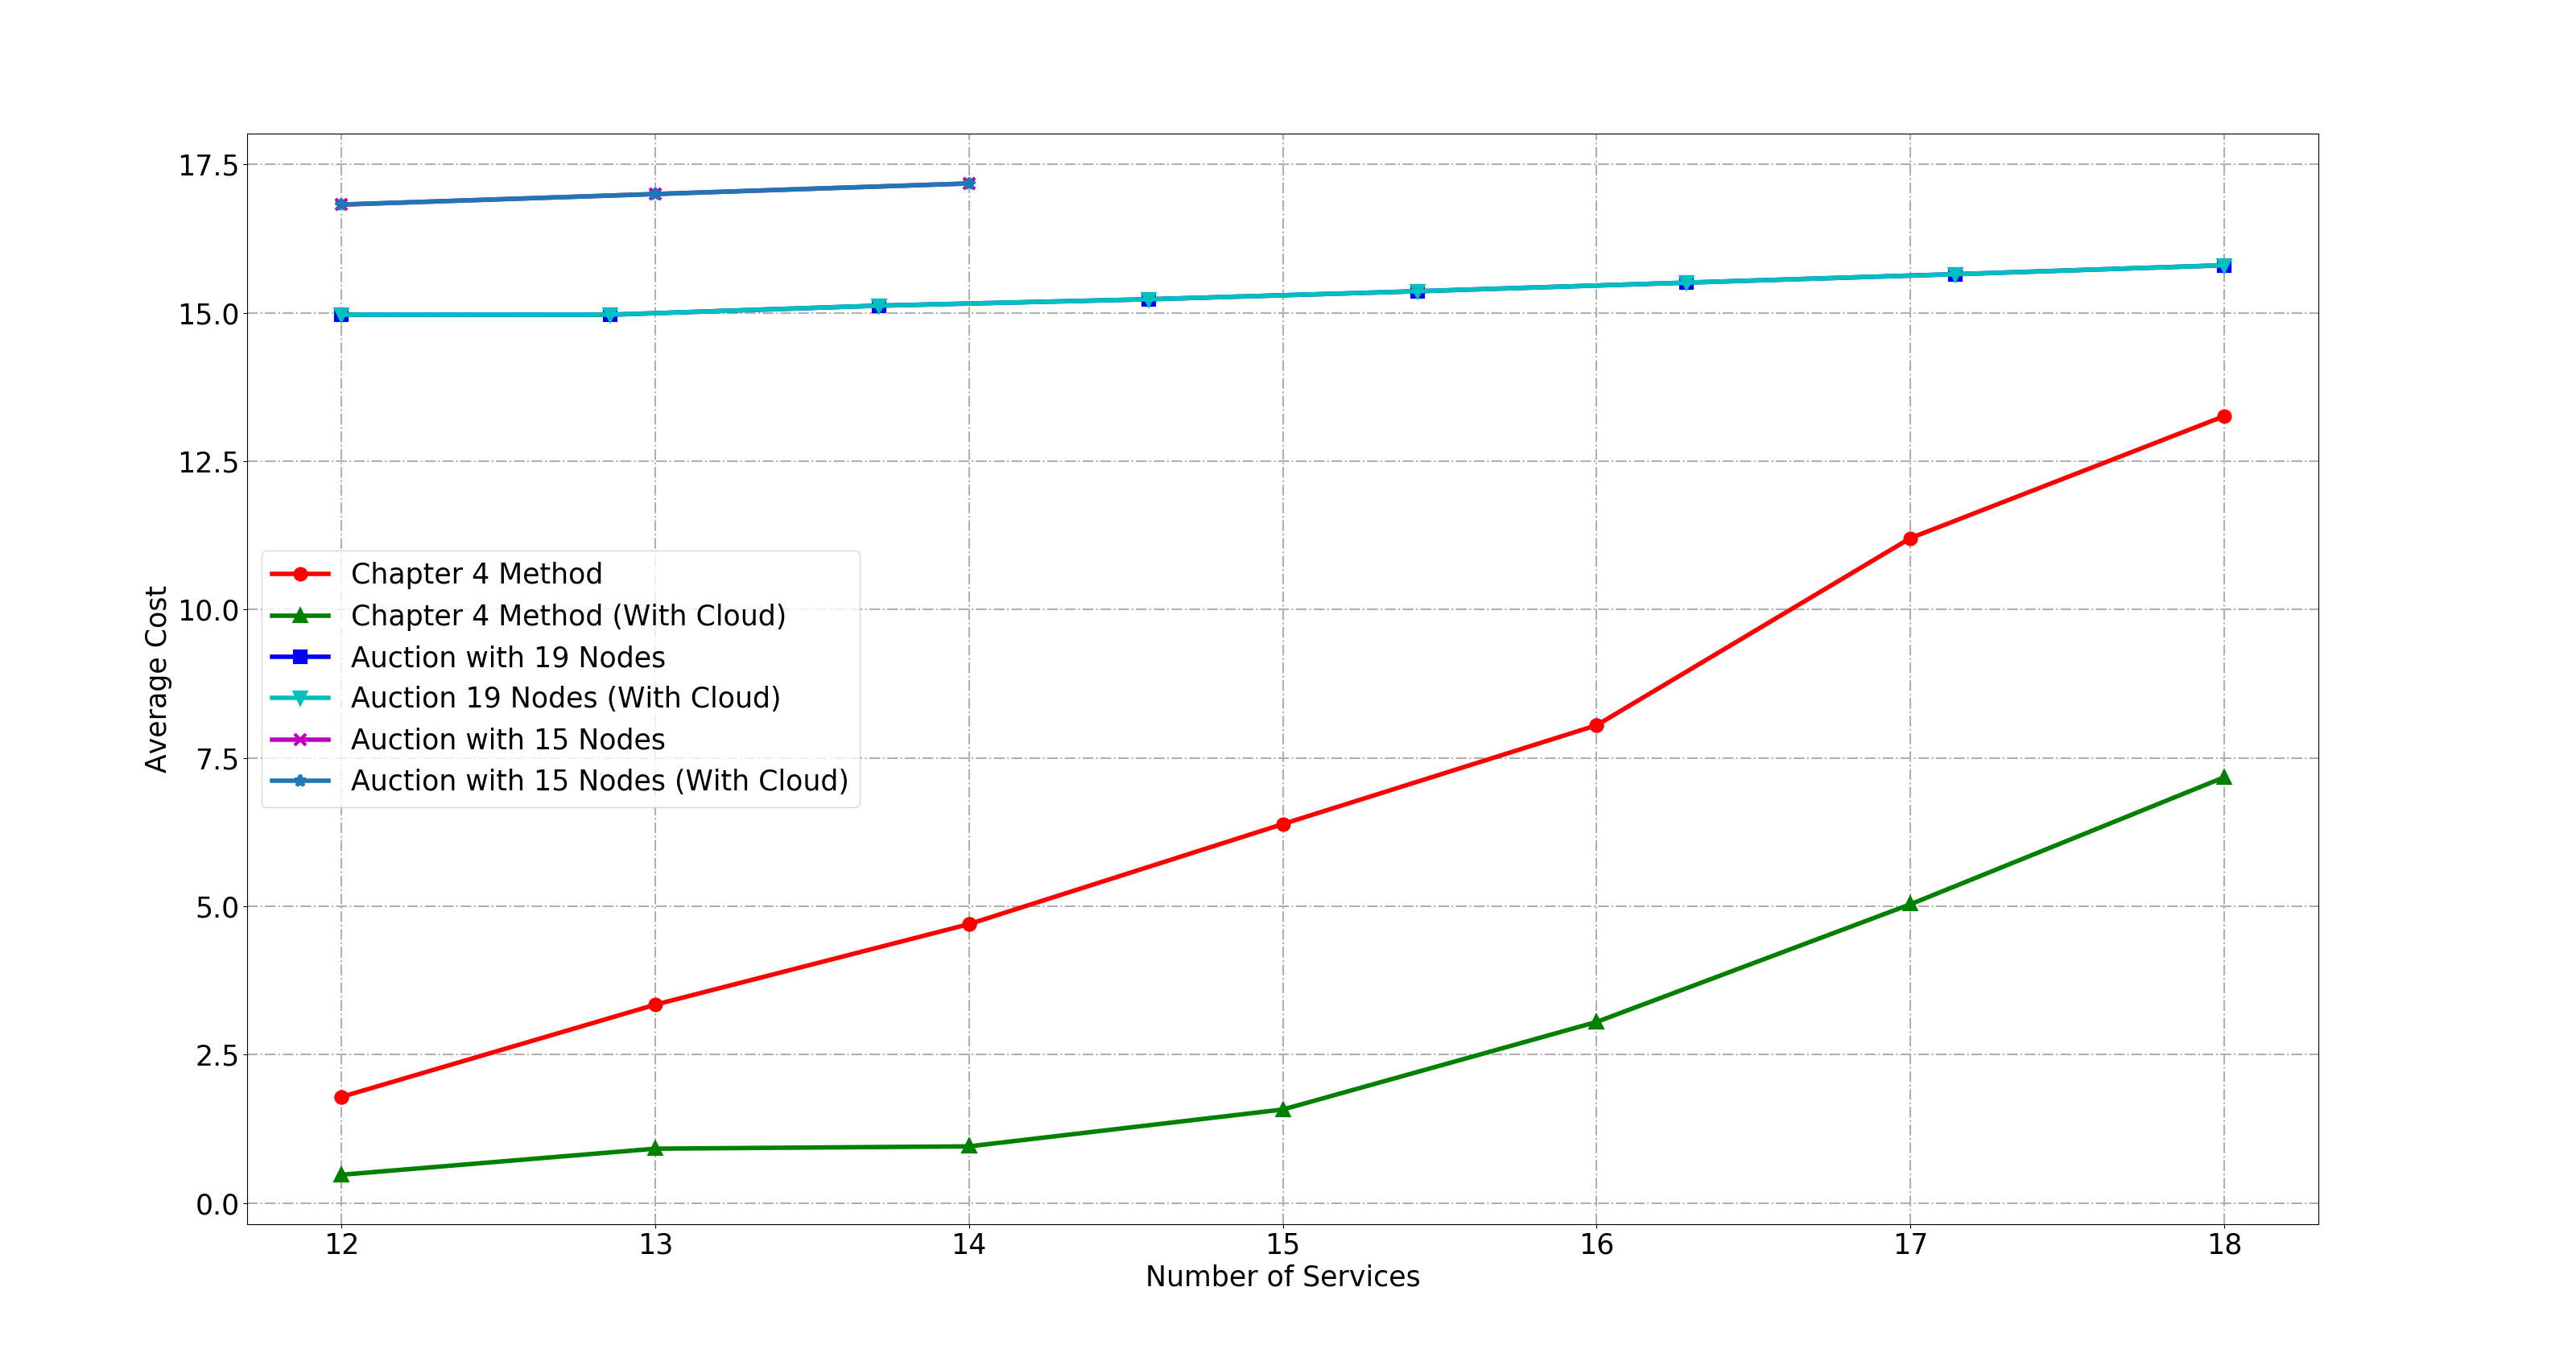
\includegraphics[width=17cm]{graphics/many_to_many/sim_9}}
      \caption{تاثیر تعداد سرویس‌ها بر میانگین هزینه سرویس‌ها}
      \label{fig:many_to_many:sim9}
    \end{figure}

    در شبیه سازی بعدی فرض می‌کنیم که تعداد منابع پردازشی ثابت و برابر ۱۵ باشد و تعداد سرویس‌ها در بازه‌ی $[12,18]$ تغییر کند.
    برای مقایسه، نتایج حاصل از الگوریتم مبتنی مزایده آورده شده است.
    چون در الگوریتم مبتنی بر مزایده باید تعداد سرویس‌ها کم‌تر از تعداد منابع پردازشی باشد، نتایج الگوریتم مبتنی بر مزایده در دو حالت آورده شده است.
    در حالت اول، تعداد منابع بیش‌تر از حداکثر تعداد سرویس‌ها است و مقایسه در کل بازه رسم شده‌است.
    در حالت دوم، تعداد منابع، برابر ۱۵ است، به همین دلیل نتایج فقط برای تعداد سرویس‌های کم‌تر قابل محاسبه بوده است.
    با توجه به شکل، واضح است که الگوریتم معرفی شده در این فصل به نتایج بسیار بهتری نسبت به الگوریتم تخصیص منابع مبتنی بر مزایده می‌رسد.
    به دلیل این که تعداد منابع پردازشی ثابت است، انتظار داریم افزایش تعداد سرویس‌ها باعث افزایش هزینه میانگین سرویس‌هایی که از ابتدا در سیستم وجود داشتند شود.
    در \cref{fig:many_to_many:sim9} میانگین هزینه‌ی ۱۲ سرویس اول را برای تعداد سرویس‌های شبیه‌سازی شده رسم کرده‌ایم.
    در این شکل مطابق انتظار با افزایش تعداد سرویس‌ها، میانگین هزینه سرویس‌هایی که از ابتدا در سیستم قرار داشتند افزایش پیدا کرده‌است.
    علاوه بر این مانند بقیه شبیه‌سازی‌ها، در سناریو‌ای که دارای منبع پردازشی ابری است، میانگین هزینه ۱۲ سرویس اول کم‌تر از سناریو‌ی بدون منبع پردازشی ابری است.
    هم‌چنین با افزایش تعداد سرویس‌ها، اختلاف این دو سناریو افزایش پیدا می‌کند، چراکه منبع پردازشی ابری ظرفیت پردازشی بالایی دارد و سرویس‌ها با استفاده از آن هزینه‌ی خود را کاهش می‌دهند.

  \section{جمع‌بندی و نتیجه‌گیری}
    در این فصل مسئله تخصیص منابع پردازشی به صورت چند به چند برای سرویس‌های اینترنت اشیاء بررسی شد.
    در این نوع از تخصیص منابع، هر سرویس می‌تواند از چند منبع پردازشی استفاده کند و منابع پردازشی هم می‌توانند به چند سرویس اختصاص پیدا کنند.
    ابتدا این مسئله به صورت یک مسأله برنامه‌ریزی غیرخطی عدد صحیح مخلوط فرمول بندی شد.
    با توجه به پیچیدگی حل مسئله ارائه شده، یک روش زیر بهینه برای حل آن ارائه شد.
    پس از آن نتایج شبیه‌سازی الگوریتم ارائه شده بررسی شد.

